\chapter{任务目标}

本次课程设计的任务是基于谣言检测数据集,构建一个检测模型。该模型可以对数据集中的推文进行谣言检测与识别。要求如下:
\begin{itemize}
    \item 数据集:使用给定的谣言检测数据集,数据集包含推文文本和标签(谣言或非谣言)。
    \item 训练模型:使用逻辑回归或GRU等深度学习模型进行谣言检测,实现二分类任务,
    用0代表非谣言、1代表谣言
    \item 泛化能力:模型应具有较好的泛化能力,能够适应不同类型的谣言检测任务。
    \item 评估指标:分类准确率、运行时间等
    \item 结果可视化:对模型训练结果进行可视化展示。
\end{itemize}

\vspace{1em}

我们需要在接口类文件classify.py中实现接口类RumourDetectClass,该类对外提供一个接口函数classify,该函数接收一条字符串作为输入,输出一个int值作为对应的预测类别。该类共包含以下方法:
\begin{itemize}
    \item \verb|__init__(self, model_path, vocab_path, EMBEDDING_DIM = 128, |\\
    \verb|HIDDEN_DIM = 256, DEVICE = NONE)|: 初始化,加载指定词表和模型参数
    \item \verb|construct_detector(self)|: 无参数快速构建谣言检测器,加载默认模型和词表
    \item \verb|classify(self, text)|: 对输入文本进行预测,返回预测结果
\end{itemize}

\chapter{具体内容}

\section{实施方案}

在经过小组成员的讨论后,我们决定采用AdvancedBiLSTM3(改进型双向长短时记忆网络)模型开展谣言检测任务。该模型在传统BiLSTM基础上,结合了注意力机制、Dropout正则化和LayerNorm等技术,能够更好地捕捉文本的上下文依赖关系,并有效缓解过拟合问题。具体方案如下:

\vspace{1em}
首先,我们对数据进行预处理:
\begin{itemize}
    \item \textbf{构建数据集}:除了老师给定的训练集和测试集外,我们还从PHEME Dataset额外获取到更多的推特谣言数据集,经过分类处理后按照8:1:1的比例划分为训练集、验证集和测试集。训练集包含约5500条推文,验证集和测试集各包含约600条推文。
    \item \textbf{文本清洗}:使用正则表达式去除URL和@提及,统一转换为小写,并通过NLTK进行分词和词干提取,降低词形变化对模型的干扰。
    \item \textbf{词表构建}:基于训练集文本构建词表,过滤低频词(最小频率2),并添加\verb|<PAD>|(填充符)和\verb|<UNK>|(未知词)标记。
    \item \textbf{序列编码}:将文本转换为固定长度的数字序列(\verb|MAX_LEN=64|),不足长度的文本使用\verb|<PAD>|进行填充,超长部分截断(采用前向截断),确保输入数据的一致性。
\end{itemize}

\vspace{1em}
在模型架构上,我们采用的AdvancedBiLSTM3模型包含以下关键模块:
\begin{itemize}
    \item \textbf{嵌入层}:使用可训练的词向量,维度为\verb|EMBEDDING_DIM=128|,并在嵌入层后添加\verb|Dropout|以缓解过拟合。
    \item \textbf{双向LSTM层}:使用双向LSTM,设置\verb|bidirectional=True|,并设置隐藏层维度为\verb|HIDDEN_DIM=256|以捕捉上下文语义。此外还采用2层堆叠结构,并在层间使用\verb|Dropout|。
    \item \textbf{注意力机制}:引入多层注意力机制,通过\verb|Tanh|激活函数和128维的中间层增强特征表达,使用掩码处理填充值,避免无效位置参与注意力计算。
    \item \textbf{分类器}:包含多层全连接网络,使用\verb|ReLU|激活函数和\verb|LayerNorm|归一化,最终通过\verb|sigmoid|函数输出二分类结果,即以0表示非谣言,1表示谣言。
\end{itemize}

\vspace{1em}
模型训练过程中,我们采用以下策略:
\begin{itemize}
    \item \textbf{优化器}:使用Adam优化器,初始学习率\verb|LEARNING_RATE=0.009|,结合学习率衰减策略(\verb|ReduceLROnPlateau|),当验证集F1分数不再提升时,学习率按因子\verb|FACTOR=0.9|衰减,衰减耐心值为3轮。
    \item \textbf{损失函数}:采用\verb|BCEWithLogitsLoss|(二元交叉熵损失),内置\verb|sigmoid|激活,支持批量二分类任务。
    \item \textbf{正则化}:为防止模型过拟合,增加权重衰减\verb|WEIGHT_DECAY=1e-4|,并结合多层\verb|Dropout|在嵌入层、LSTM层和全连接层中进行正则化。
    \item \textbf{数据增强}:合并原始训练集与新增训练集,总训练样本量提升至约5500条数据,验证集同步合并以增强泛化性。
\end{itemize}  

\vspace{1em}
与传统的BiGRU或逻辑回归模型相比,AdvancedBiLSTM3模型具备更强的特征表达能力和鲁棒性,能够自动学习文本中的复杂语义关系,适应不同领域的谣言检测任务。通过注意力机制,模型能够聚焦于文本中的关键信息片段,提升对谣言特征的捕捉能力。在对比不同策略的训练成果后,我们发现该模型在准确率和泛化能力方面均优于传统方法,具体的实验结果将在后续章节中详细展示。

\newpage
\section{核心代码分析}

\subsection{模型定义model.py}
\begin{codeblock}[language=Python]
import torch
import torch.nn as nn
class AdvancedBiLSTM3(nn.Module):  
    def __init__(self, vocab_size, embedding_dim, hidden_dim, num_layers=2, dropout=0.5):  
        super().__init__()  
        self.embedding = nn.Embedding(vocab_size, embedding_dim, padding_idx=0)  
        # 嵌入层Dropout增强鲁棒性  
        self.embedding_dropout = nn.Dropout(dropout + 0.1) 
        self.lstm = nn.LSTM(  
            embedding_dim,  
            hidden_dim // 2,
            num_layers=min(num_layers, 2),  
            bidirectional=True,  
            batch_first=True,  
            dropout=dropout if num_layers > 1 else 0  
        )  
        # 带中间层的注意力机制  
        self.attention = nn.Sequential(  
            nn.Linear(hidden_dim, 128),  
            nn.Tanh(),  
            nn.Dropout(dropout),  
            nn.Linear(128, 1)  
        )  
        # 带正则化的分类器  
        self.classifier = nn.Sequential(  
            nn.Dropout(dropout + 0.1),  
            nn.Linear(hidden_dim, 64),  
            nn.ReLU(),  
            nn.LayerNorm(64),  
            nn.Dropout(dropout),  
            nn.Linear(64, 1)  
        )  
\end{codeblock}

在模型定义中,我们通过\verb|hidden_dim//2|设置双向LSTM的隐藏层维度,确保模型能够捕捉到文本的双向上下文信息。此外我们还引入带中间层的注意力机制,通过\verb|Tanh|激活函数和128维的中间层增强特征表达,使用掩码处理填充值,避免无效位置参与注意力计算。分类器则包含多层全连接网络,使用\verb|ReLU|激活函数和\verb|LayerNorm|归一化,最终通过\verb|sigmoid|函数输出二分类结果。

\vspace{1em}
\subsection{训练模型train\_lstm.py}
\begin{codeblock}[language=Python]
import torch
import torch.nn as nn
import torch.optim as optim
from torch.utils.data import Dataset, DataLoader
import pandas as pd
from collections import Counter
import re
import joblib
import matplotlib.pyplot as plt
from sklearn.metrics import precision_score, recall_score, f1_score, confusion_matrix, classification_report
import numpy as np
from nltk.tokenize import word_tokenize
from nltk.stem import PorterStemmer
from model import AdvancedBiLSTM3 as AdvancedBiLSTM

# 超参数设置
BATCH_SIZE = 32         # 批大小
EMBEDDING_DIM = 128     # 嵌入维度(可修改)
HIDDEN_DIM = 256        # 隐藏层维度(可修改)
EPOCHS = 30             # 训练轮数(可修改)
MAX_LEN = 64            # 文本最大长度
LEARNING_RATE = 0.9e-2  # 学习率(可修改)
FACTOR = 0.9            # 学习率衰减因子
WEIGHT_DECAY = 1e-4     # L2正则化
DEVICE = torch.device('cuda:0' if torch.cuda.is_available() else 'cpu') 

# 路径设置
model_parameter = f'{EMBEDDING_DIM}_{HIDDEN_DIM}_{EPOCHS}_{LEARNING_RATE}'
model_path = f'../Output/Model/{model_parameter}.pt'
vocab_path = f'../Output/Model/vocab_{model_parameter}.pkl'
train_path = '../Dataset/split/train.csv'
ex_train_path = '../Dataset/split/ex_train.csv'
val_path = '../dataset/split/val.csv'
ex_val_path = '../dataset/split/ex_val.csv'
test_path = '../dataset/test/test.csv'
graph_path = f'../Output/Graph/{model_parameter}.png'

def tokenize(text):
    """对文本进行分词和预处理"""
    # 处理URL和@提及
    text = re.sub(r'http\S+', '<URL>', text)
    text = re.sub(r'@\w+', '@USER', text)
    # 使用NLTK分词+词干提取
    tokens = word_tokenize(text)
    stemmer = PorterStemmer()
    return [stemmer.stem(w.lower()) for w in tokens if w.isalpha()]

def build_vocab(texts, min_freq=2):
    """构建词表,与示例代码相同"""
    pass

def encode(text, vocab):
    """将文本编码为数字序列,与示例代码相同"""
    pass

class RumorDataset(Dataset):
    """自定义数据集类,与示例代码相同"""
    pass
    
def evaluate(model, loader):
    """评估函数,调用外部库计算返回准确率、精确率、召回率和F1-score"""
    pass

def plot_learning_curve(train_metrics, val_metrics, epochs, save_path):
    """绘制包含损失率和核心指标的双图学习曲线"""
    pass

def main():
    # 读取数据集
    print("正在加载数据...")
    train_df = pd.read_csv(train_path)
    ex_train_df = pd.read_csv(ex_train_path)  # 读取新增训练集
    print(f"ex训练集大小: {len(ex_train_df)}")
    print(f"原始训练集大小: {len(train_df)}")
    train_df = pd.concat([train_df,ex_train_df], ignore_index=True)
    print(f"合并后的训练集大小: {len(train_df)}")
    val_df = pd.read_csv(val_path)
    ex_val_df = pd.read_csv(ex_val_path)
    print(f"验证集大小: {len(val_df)}")
    print(f"新增验证集大小: {len(ex_val_df)}")
    val_df = pd.concat([val_df,ex_val_df], ignore_index=True)
    print(f"合并后的验证集大小: {len(val_df)}")

    # 构建词表
    print("正在构建词表...")
    vocab = build_vocab(train_df['text'])
    joblib.dump(vocab, vocab_path)  # 保存词表
    
    # 构建数据集
    train_set = RumorDataset(train_df, vocab)
    val_set = RumorDataset(val_df, vocab)

    train_loader = DataLoader(train_set, batch_size=BATCH_SIZE, shuffle=True)
    val_loader = DataLoader(val_set, batch_size=BATCH_SIZE)

    # 初始化模型、优化器和损失函数
    print("正在初始化模型...")
    model = AdvancedBiLSTM(len(vocab), EMBEDDING_DIM, HIDDEN_DIM).to(DEVICE)
    optimizer = optim.Adam(model.parameters(), lr=LEARNING_RATE)
    scheduler = optim.lr_scheduler.ReduceLROnPlateau(
    optimizer, mode='max', factor=FACTOR, patience=3, verbose=True
    )
    criterion = nn.BCEWithLogitsLoss()

    # 记录训练过程指标
    train_history = {
        'loss': [], 'accuracy': [], 'precision': [], 'recall': [], 'f1': []
    }
    val_history = {
        'loss': [], 'accuracy': [], 'precision': [], 'recall': [], 'f1': []
    }
    print("开始训练模型...")
    # 训练模型
    best_val_f1 = 0.0
    for epoch in range(EPOCHS):
        model.train()
        epoch_loss = 0
        # 训练一个epoch
        for x, y in train_loader:
            x, y = x.to(DEVICE), y.to(DEVICE)
            logits = model(x)
            loss = criterion(logits, y)
            optimizer.zero_grad()
            loss.backward()
            optimizer.step()
            epoch_loss += loss.item()   
        avg_loss = epoch_loss / len(train_loader)

        # 计算训练集指标
        train_acc, train_prec, train_rec, train_f1, _ = evaluate(model, train_loader)
        train_history['accuracy'].append(train_acc)
        train_history['precision'].append(train_prec)
        train_history['recall'].append(train_rec)
        train_history['f1'].append(train_f1)
        train_history['loss'].append(avg_loss)

        val_acc, val_prec, val_rec, val_f1, val_loss = evaluate(model, val_loader)
        val_history['accuracy'].append(val_acc)
        val_history['precision'].append(val_prec)
        val_history['recall'].append(val_rec)
        val_history['f1'].append(val_f1)
        val_history['loss'].append(val_loss)
        
        scheduler.step(val_f1)  # 根据验证集F1分数调整学习率
        
        print(f'Epoch {epoch+1}/{EPOCHS}')
        # 保存最佳模型
        if val_f1 > best_val_f1:
            best_val_f1 = val_f1
            torch.save(model.state_dict(), model_path)
            print(f'Saved best (Train F1: {val_f1:.4f})')
        print(f'Train: Loss={avg_loss:.4f}, Acc={train_acc:.4f}, Prec={train_prec:.4f}, Rec={train_rec:.4f}, F1={train_f1:.4f}')
        print(f'Val: Loss={val_loss:.4f}, Acc={val_acc:.4f}, Prec={val_prec:.4f}, Rec={val_rec:.4f}, F1={val_f1:.4f}')
        print('-' * 60)
    print("\n 训练完成!")
    plot_learning_curve(train_history, val_history, EPOCHS, graph_path)
    
if __name__ == '__main__':
    main()
\end{codeblock}

在训练模型的代码中,我们首先定义了超参数和路径设置,接着使用\verb|tokenize|函数对文本进行分词和预处理,\verb|build_vocab|函数构建词表,并将其保存到指定路径。然后,我们定义了自定义数据集类\verb|RumorDataset|,用于加载和处理数据。接下来,我们初始化模型、优化器和损失函数,并记录训练过程中的指标。通过循环迭代训练数据,计算损失并更新模型参数,同时在每一轮训练结束后评估模型在验证集上的性能。最终,我们将最佳模型参数保存到指定路径,并绘制学习曲线。

\vspace{1em}
\subsection{接口类定义classify.py}
\begin{codeblock}[language=Python]
import torch
import joblib
from model import AdvancedBiLSTM3 as AdvancedBiLSTM 
from train_lstm import *

class RumourDetectClass:
    def __init__(self, model_path, vocab_path, embedding_dim=EMBEDDING_DIM, hidden_dim=HIDDEN_DIM, device=DEVICE):
        # 加载词表和模型参数
        self.vocab = joblib.load(vocab_path)
        self.model = AdvancedBiLSTM(len(self.vocab), embedding_dim, hidden_dim).to(device)
        self.model.load_state_dict(torch.load(model_path, map_location=device))
        self.model.eval()

    @classmethod
    def construct_detector(cls):
        embedding_dim = EMBEDDING_DIM
        hidden_dim = HIDDEN_DIM
        epochs = EPOCHS
        learning_rate = LEARNING_RATE
        device = DEVICE
        model_path = f'../Output/Model/best_{embedding_dim}_{hidden_dim}_{epochs}_{learning_rate}.pt'
        vocab_path = f'../Output/Model/vocab_{embedding_dim}_{hidden_dim}_{epochs}_{learning_rate}.pkl'
        return cls(model_path, vocab_path, embedding_dim, hidden_dim, device)

    
    def classify(self, text: str) -> int:
        # 预测流程
        ids = encode(text, self.vocab)
        x = torch.tensor([ids], dtype=torch.long).to(DEVICE)
        with torch.no_grad():
            logits = self.model(x)
            pred = (torch.sigmoid(logits) > 0.5).float().item()
        return int(pred)
\end{codeblock}

在接口类中,我们实现了\verb|RumourDetectClass|接口类,该类提供了两个初始化方法:\verb|__init__|和\verb|construct_detector|,分别可以进行指定或默认模型和词表的初始化谣言检测器。此外还实现了一个接口函数\verb|classify|,接收一条字符串作为输入,输出一个整数值作为对应的预测类别。通过\verb|construct_detector|方法,我们可以快速构建谣言检测器,加载默认模型和词表。

\vspace{1em}
本项目代码发布在\href{https://github.com/youyeyejie/NIS4307_RumorDetect.git}{GitHub} 和 \href{https://git.sjtu.edu.cn/ma_yuezhao/nis4307_rumordetect}{GitSJTU} 上,包含了数据预处理、模型训练、模型评估和接口类的完整实现。

\newpage
\section{测试结果分析}

在确定模型架构后,我们经过不断调整训练时使用的参数,最终选定了以下配置:
\begin{itemize}
    \item 嵌入维度:\verb|EMBEDDING_DIM = 128|
    \item 隐藏层维度:\verb|HIDDEN_DIM = 256|
    \item 训练轮数:\verb|EPOCHS = 30|
    \item 学习率:\verb|LEARNING_RATE = 0.009|
    \item 批大小:\verb|BATCH_SIZE = 32|
    \item 最大文本长度:\verb|MAX_LEN = 64|
    \item 学习率衰减因子:\verb|FACTOR = 0.9|
    \item L2正则化:\verb|WEIGHT_DECAY = 1e-4|
\end{itemize}

在经过30轮训练后,我们得到了如下图\ref{fig:learning_curve}所示的模型训练指标,30轮训练总耗时约5分钟,最佳模型在第21轮产生,其验证集F1分数达到了0.8592。可以看到,随着训练轮数的增加,训练集和验证集的损失率逐渐波动降低,验证集的准确率、精确率、召回率和F1分数也在不断波动提升,表明模型在谣言检测任务上取得了较好的效果。
\vspace{-0.2cm}
\begin{figure}[ht]
  \centering
  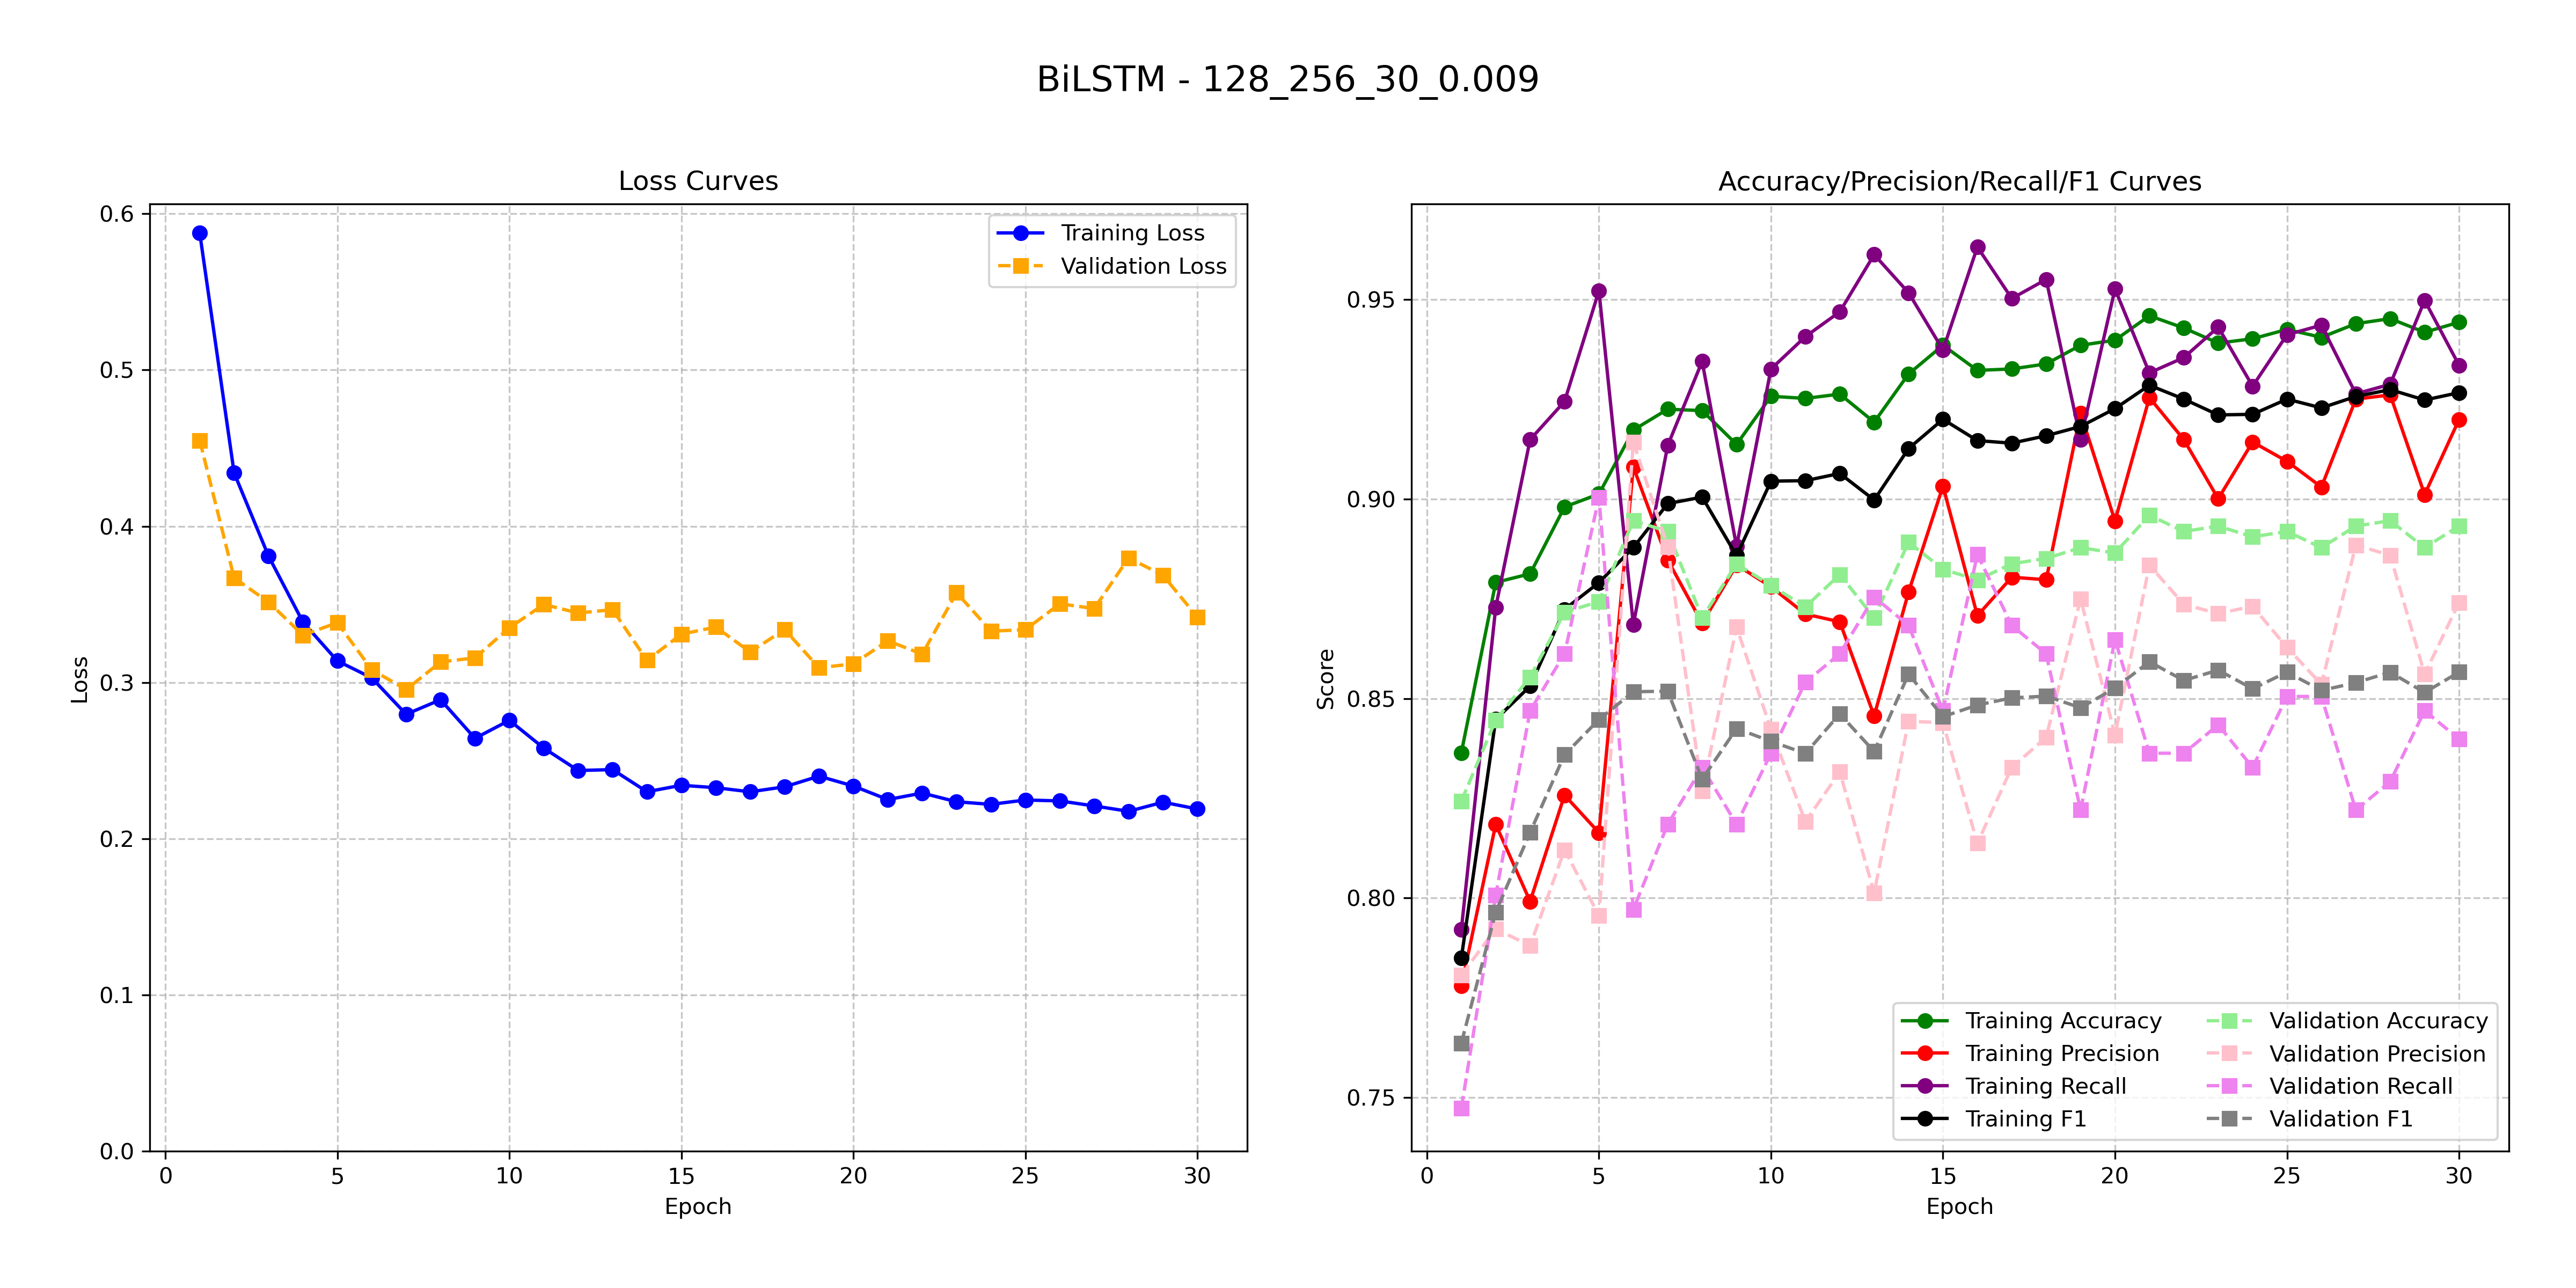
\includegraphics[width=0.8\textwidth]{../Output/Graph/best_128_256_30_0.009.png}
  \caption{模型训练过程中的损失率和核心指标的双图学习曲线}
  \label{fig:learning_curve}
\end{figure}

使用test.py脚本对测试集进行评估,我们得到了如下表\ref{tab:test_results}所示的测试结果。结果表明,此模型在我们的测试集上表现良好,其中预测准确率达到了86.64\%。
\begin{table}[ht]
\centering
\begin{tabular}{|c|c|c|}
\hline
预测 \textbackslash{} 真实 & 非谣言(0) & 谣\quad 言(1) \\
\hline
非谣言(0) & 303 & 44 \\
\hline
谣\quad 言(1) & 28 & 164 \\
\hline
\end{tabular}
\caption{测试结果}
\label{tab:test_results}
\end{table}


\chapter{工作总结}

\section{收获与心得}

通过本次课程设计,我们深入学习了深度学习模型在自然语言处理中的应用,特别是双向门控循环单元(BiGRU)和改进型双向长短时记忆网络(AdvancedBiLSTM)模型在谣言检测任务中的应用,也深刻体会到了理解BiLSTM结合注意力机制在序列分类中的优势。通过对比不同模型的性能,我们认识到模型的选择对任务结果的影响。此外,我们实现了从数据预处理、模型训练到模型评估的全流程开发,初步掌握了如何使用PyTorch等深度学习框架进行自然语言处理任务。

\section{遇到问题及解决思路}

在项目实施过程中,我们也遇到了一些问题,例如数据集不平衡导致模型偏向于某一类标签、训练轮数过多导致出现过拟合现象、以及模型参数设置不当导致训练效果不佳等。针对这些问题,我们采取以下解决思路:
\begin{itemize}
    \item \textbf{数据集不平衡}:我们通过自行搜索PHEME Dataset等公开数据集,增加了训练集的样本量,并对数据进行分层随机抽样,确保各类标签的样本数量相对均衡,极大丰富了数据集内容,从而获得更全面的训练样本。
    \item \textbf{过拟合问题}:针对较多训练轮数中验证集损失曲线先降后升的过拟合问题,我们引入了Dropout正则化技术,并通过交叉验证选择最佳模型参数,避免模型在训练集上过拟合。
    \item \textbf{模型参数设置}:在实验过程中,我们不断调整模型参数,如学习率、嵌入维度、隐藏层维度等,尝试不同的网络结构和超参数组合。通过对比不同配置下的模型性能,我们最终找到了在有限时间内训练出较为稳定模型的佳配置。
\end{itemize}

\vspace{1em}
通过这些问题的解决,我们不仅提升了模型的性能,也加深了对深度学习模型在自然语言处理任务中应用的理解。
    
\chapter{课程建议}

本次课程设计通过实践操作,让我们对深度学习与自然语言处理的结合应用有了具象认知,但在课程学习及实践过程中,也发现一些可以优化改进的方向,此处提出几点建议,希望能为后续课程设计提供参考:

当前课程较多聚焦于基础概念的介绍讲解,但对具体算法的原理推导与代码实现讲解较少,部分概念比较晦涩难懂但缺乏深入剖析,导致学生在理解上存在困难。希望老师能结合代码实例进行拆解演示,如结合 PyTorch 等库的具体实现,深入讲解 GRU、LSTM 等模型的工作原理与数学推导,帮助学生更好地理解模型背后的逻辑。

此外,本课程前期未铺垫相关实践案例,而课程设计在学期末才公布,与其他课程结课任务、考试复习等时间冲突,导致学生难以分配足够精力深入探索,也是我认为可以改进的地方。在本次课程设计中,我们小组成员普遍感受到时间紧迫,从理解任务、数据预处理到模型调优全程压缩在短时间内,尤其是在数据预处理、模型训练与调优等环节,难以进行充分的实验与探索。建议将课程设计主题提前半学期公布,分阶段设置任务节点(如第 8 周完成数据预处理、第 12 周提交模型初版等),并配套阶段性指导,帮助学生合理规划时间,确保实践质量。

而在完成项目的过程中,我们也意识到仅凭课堂上学到的知识,难以独立完成整个项目,特别是对 PyTorch 、Sklearn 等库的使用不够熟悉,导致在实现过程中遇到很多问题。建议老师能在前期的课程中结合具体案例,帮助学生更好地掌握这些工具的使用方法。